\section{\Sys's Overview}
\label{sec:overview}

\begin{figure*}[t]
    \centering
    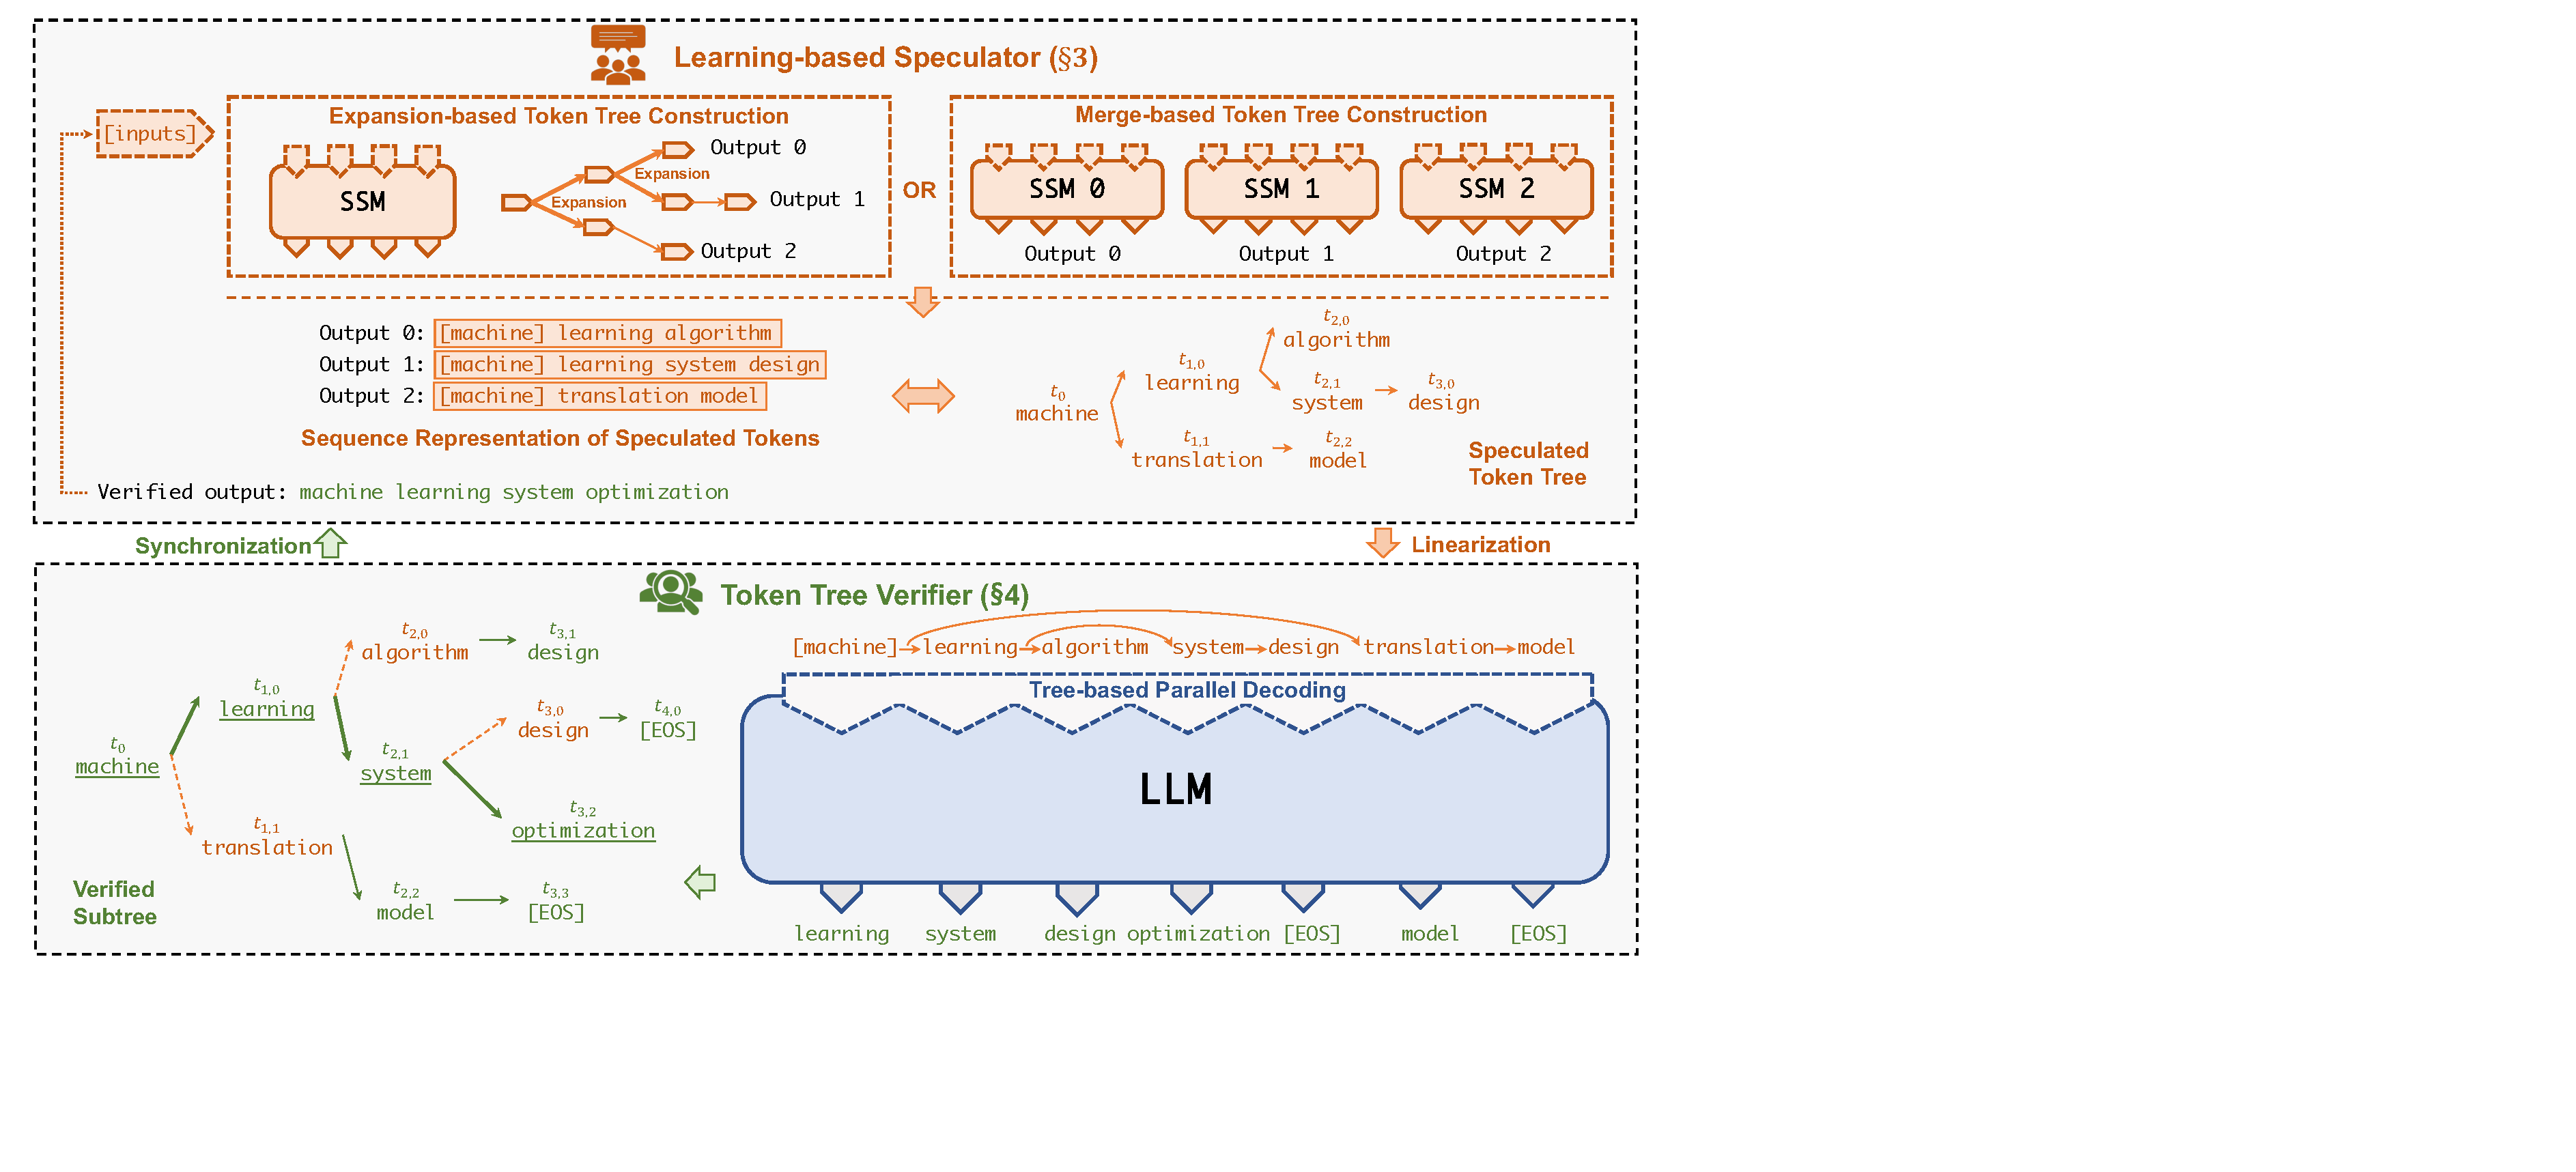
\includegraphics[scale=0.4]{rebuttal_figs/speculative_inference_overview9.pdf}
    \caption{An overview of \Sys's tree-based speculative inference and verification mechanism.}
    \label{fig:speculative_inference}
\end{figure*}


\begin{algorithm}
%\small
\caption{The incremental decoding algorithm used in existing LLM serving systems.}
\label{alg1}
\begin{algorithmic}[1]
\State {\bf Input:} A sequence of input tokens $\m{I}$
\State {\bf Output:} A sequence of generated tokens
\State $\m{S} = \m{I}$
\While{true}
\State $t = \Call{Decode}{\textrm{LLM}, \m{S}}$
\State $\m{S}$.append($t$)
\If{$t = \langle \textrm{EOS} \rangle$}
\State {\bf Return} $\m{S}$
\EndIf
\EndWhile
\end{algorithmic}
\end{algorithm}


\begin{algorithm}
%\small
\caption{The speculation and verification algorithm used by \Sys. \textproc{Speculate} takes the current token sequence $\m{S}$ as an input and generates a speculated token tree $\m{N}$. 
\textproc{TreeParallelDecode} generates a token $\m{O}(u)$ for each node $u \in \m{N}$.
%\Sys's use of an LLM is different from existing systems: the LLM takes a token tree $\m{N}$ as an input and generates a token $\m{O}(u)$ for each node $u \in \m{N}$. Note that the \textproc{TreeParallelDecode} function can generate all tokens in $\m{O}$ in a single LLM decoding step (see~\Cref{sec:verification}).
\textproc{VerifyGreedy} and \textproc{VerifyStochastic} examine $\m{N}$ against $\m{O}$ and produce a sequence of verified tokens $\m{V}$ using greedy or stochastic sampling, respectively.}
%\caption{The speculative inference and token tree verification algorithm used by \Sys.}
\label{alg2}
\begin{algorithmic}[1]
\State {\bf Input:} A sequence of input tokens $\m{I}$
\State {\bf Output:} A sequence of generated tokens
\State $\m{S} = \m{I}$
\While{true}
\State $\m{N} = \Call{Speculate}{\m{S}}$
\State $\m{O} = \Call{TreeParallelDecode}{\textrm{LLM}, \m{N}}$ 
%\XM{How about using a function that takes LLM as input to highlight the differences of using LLMs? E.g., t$\gets$Decode(LLM, S) for Algorithm 1 and $\m{O}\gets$ParallelDecode(LLM, $\m{N}$) in Algorithm 2}
\If{use greedy decoding}
\State $\m{V} = \Call{VerifyGreedy}{\m{O}, \m{N}}$
\Else
\State $\m{V} = \Call{VerifyStochastic}{\m{O}, \m{N}}$
\EndIf
\For{$t \in \m{V}$}
\State $\m{S}$.append($t$)
\If{$t = \langle \textrm{EOS} \rangle$}
\State {\bf return} $\m{S}$
\EndIf
\EndFor
\EndWhile
\State

\Function{VerifyGreedy}{$\m{O}, \m{N}$}
\State $\m{V} = \emptyset$, $u \leftarrow$ the root of token tree $\m{N}$
\While{$\exists v \in \m{N}. p_v = u \textrm{ and } t_v = \m{O}(u)$}
\State $\m{V}$.append($t_v$) 
\State $u = v$ 
\EndWhile
\State $\m{V}$.append($\m{O}(u)$)
\State {\bf return} $\m{V}$
\EndFunction
\State

\Function{VerifyStochastic}{$\m{O}, \m{N}$}
\State $\m{V} = \emptyset$, $u \leftarrow$ the root of token tree $\m{N}$
\While{$u$ is a non-leaf node}
%\State $\m{H} = \textrm{child}(u), P(x)\coloneqq P(x \mid u, \Theta_{\textrm{LLM}})$ 
\State $\m{H} = \textrm{child}(u)$
\Comment{\textcolor{violet}{The set of child nodes for $u$}}
    \While{$\m{H}$ is not empty}
    % \Comment{get $q_{i}(\cdot\mid u)$ with the smallest total variation distance w.r.t $p(\cdot\mid u)$}
    \State $s\sim \textrm{rand}(\m{H}), r \sim U(0, 1), x_s=\m{H}[s]$ 
        \If{$r \leq {P(x_s \mid u, \Theta_{LLM})} / {P(x_s \mid u, \Theta_{SSM_s})}$}
            \LineComment{\textcolor{violet}{Token $x_s$ passes verification.}}
            \State $\m{V}$.append($x_s$)
            \State $u = s$
            \State {\bf break}
        \Else            
            \LineComment{\textcolor{violet}{Normalize the residual $P(x \mid u, \Theta_{LLM})$}}
            % \LineComment{normalize the residual distribution between $q(x \mid u)$ and $p(x \mid u)$}
            \State $P(x \mid u, \Theta_{\textrm{LLM}})\coloneqq \textrm{norm}(\max(0, P(x \mid u, \Theta_{\textrm{LLM}})-P(x \mid u, \Theta_{\textrm{SSM}_s})))$ 
            \State $\m{H}.\textrm{pop}(s)$
        \EndIf   
    \EndWhile
\If{$\m{H}$ is empty}
    \State {\bf break}
\EndIf
\EndWhile
\LineComment{All SSMs fail verification; sample the next token}
\State $x_{\textrm{next}} \sim P(x \mid u, \Theta_{LLM})$
\State $\m{V}$.append($x_{\textrm{next}}$)
\State {\bf return} $\m{V}$

\EndFunction
\end{algorithmic}
\end{algorithm}

% \Cref{fig:specinfer_compared_to_incr_decoding} shows an overview of \sys in comparison with incremental decoding.
\Cref{fig:speculative_inference} shows an overview of \sys, which
includes a {\em learning-based speculator} that takes as input a sequence of tokens, and produces a {\em speculated token tree}.
%%%
The goal of the speculator is to predict the LLM's output by maximizing the overlap between the speculated token tree and the tokens generated by the LLM using incremental decoding (Alg.~\ref{alg1}).
%tokens that will be generated by the LLM and maximizes the likelihood that the speculated token tree includes the true token sequence.
%%%
% As shown at the top of \Cref{fig:speculative_inference}, the speculator combines multiple distilled and/or pruned versions of the LLM, which we call small speculative models (SSMs).\XM{TODO: update}
%%%

There are several ways to prepare SSMs for speculative inference. 
First, modern LLMs generally have many smaller architectures pre-trained together with the LLM using the same datasets. 
%%%
For example, in addition to the OPT-175B model with 175 billion parameters, the OPT model family also includes OPT-125M and OPT-350M, two variants with 125 million and 350 million parameters, which were pre-trained using the same datasets as OPT-175B~\cite{zhang2022opt}.
%%%
These pre-trained small models can be directly used as SSMs. 
\rev{Second, to improve the coverage of speculated tokens from SSMs, \Sys takes an expansion-based and a merge-based speculation method as shown at the top of \Cref{fig:speculative_inference}. The speculated tokens are organized in a token tree structure.}
% \rev{\Sys takes an expansion-based mechanism for constructing a token tree from a single SSM.}
% Second, to further improve the coverage of speculated token trees, \Sys also introduces a fine-tuning technique called {\em collective boost-tuning} to cooperatively fine-tune a set of SSMs by aligning their aggregated prediction with the LLM's using adaptive boosting~\cite{freund1999short}.\XM{TODO: update}

\if 0
The speculator automatically combines the candidate token sequences predicted by individual SSMs to construct a token tree, as shown in \Cref{fig:speculative_inference}.
Since \sys executes multiple SSMs in parallel, using more SSMs does not directly increase the speculative inference latency.
%%%
However, using a large number of SSMs will result in a large token tree, which requires more memory and computation resources for verification.
%%%
To address this challenge, \sys uses a {\em learning-based} speculative scheduler to learn to decide which SSMs to use for a given input token sequence and the speculative configurations for these SSMs (e.g., the beam search width and depth when running an SSM using beam search).
\fi
%The speculation engine can be implemented as a combination of (1) user-provided functions that predict future tokens based on heuristics and/or retrieval-augmented documents, and (2) a collection of small, distilled versions of the LLM trained using the same dataset, and (3) fine-tuned versions of the small models on the target tasks.
%%%

\Sys's usage of an LLM is also different from that of existing LLM serving systems. 
Instead of using the LLM as an incremental decoder that predicts the next single token, \sys uses the LLM as a token tree verifier that verifies a speculated token tree against the LLM's output.
%%%
For each token, \sys computes its activations by considering all of its ancestors in the token tree as its preceding tokens.
%%%
For example, in \Cref{fig:speculative_inference}, the attention output of the token $t_{3,0}$ is calculated based on sequence $(t_0, t_{1,0}, t_{2, 1}, t_{3,0})$, where $t_0$, $t_{1,0}$, and $t_{2,1}$ are $t_{3,0}$'s ancestors in the token tree.
\Sys includes a novel tree-based parallel decoding mechanism to simultaneously verify {\em all} tokens of a token tree in a single LLM decoding step.

\Sys's speculative inference and token tree verification provide two key advantages over the incremental decoding approach of existing LLM inference systems.

\paragraph{Reduced memory accesses to LLM parameters.} The performance of  LLM inference is largely limited by accesses to GPU memory.
In the existing incremental decoding approach, generating a single token requires accessing all parameters of an LLM. 
%%%
The problem is exacerbated for offloading-based LLM inference systems, which use limited computational resources such as a single commodity GPU to serve LLMs by utilizing CPU DRAM and persistent storage to save model parameters and loading these parameters to GPU's high bandwidth memory (HBM) for computation.
Compared to the incremental decoding approach, \sys significantly reduces accesses to LLM parameters whenever the overlap between a speculated token tree and the LLM's actual output is not empty.
%Memory accesses to an LLM's parameters are significantly reduced when the speculation engine can correctly includes the actual future tokens in the speculated token tree.
%%%
Reduced accesses to GPU device memory and reduced data transfers between GPU and CPU memory can also directly translate to decreased energy consumption, since accessing GPU HBM consumes two or three orders of magnitude more energy than floating point arithmetic operations.

\paragraph{Reduced end-to-end inference latency.}
Serving LLMs suffers from long end-to-end inference latency.
For example, the GPT-3 architecture includes 175 billion parameters and requires many seconds to serve a request.
In the existing incremental decoding approach, the computation for generating each token depends on the keys and values of all previously generated tokens, which introduces sequential dependencies between tokens and requires modern LLM serving systems to serialize the generation of different tokens for each request.
%%%
In \sys, LLMs are used as a verifier that takes a speculated token tree as an input and can simultaneously examine {\em all} tokens in the token tree by making a single verification pass over the LLM. 
This approach enables parallelization across different tokens in a single request and reduces the LLM's end-to-end inference latency.

%\begin{itemize}
%    \item A figure to show that our approach applies to distributed inference case: (1) reduced end-to-end inference latency (2) reduced data transfers between GPUs
%    \item A figure to show that our approach applies to offload inference case: (1) reduced end-to-end inference latency (2) less memory accesses to load model weights from CPU DRAM
%\end{itemize}


